\chapter{Suunnittelu}
\label{ch:suunnittelu}
Tässä kappaleessa käydään läpi uuden järjestelmän suunnittelua. Halutun systeemin arkkitehtuuri oli esitetty aikaisemmin kuvassa \ref{fig:coupling-analysis}. Tämän osion suunnittelu koskee väliohjelmistoa ja välikättä. Suunnittelu ja päätökset pohjautuvat työssä aikaisemmin käsiteltyihin päätelmiin ja tuloksiin. Suunnittelu aloitetaan ensin antamalla kattava kokonaiskuva lukijalle. Tämän jälkeen tulevissa kappaleissa mennään tarkemmin yksityiskohtaan ja kerrotaan miten päätökset tehtiin.

% TODO: Kirjoita tähän lisää jos tarvitsee kun muu teksti on valmis.

% TODO: Asioita joihin pitää löytyä vastaus tästä kappaleesta: kielen valinta, json-viestin rakenne.

\section{Kokonaiskuva}
Suunnitellun ohjelman toiminta noudatti paljon demon toimintaperiaatteita pienin muutoksin. Kaikkien aikaisemman tiedon ja suunnitelun pohjalta päädyttiin kuvassa \ref{fig:planned-system-architecture} esitettyyn systeemin arkkitehtuuriin. Vertaa arkkitehtuuria vaatimusten pohjalta suunniteltuun arkkitehtuuriin kuvassa \ref{fig:coupling-analysis}.

\begin{figure}[ht!]
	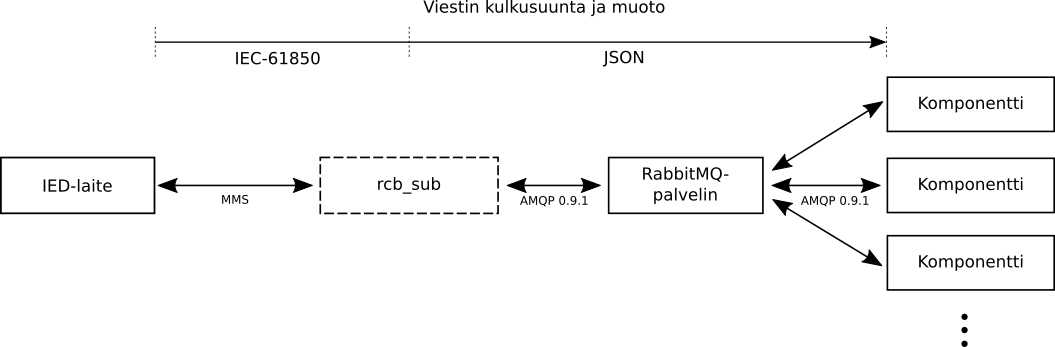
\includegraphics[width=1\textwidth]{pictures/planned-system-architecture.png}
	\caption{Suunnitellun järjestelmän arkkitehtuuri sekä viestin kulku ja muoto sen osapuolten läpi.}
	\label{fig:planned-system-architecture}
\end{figure}

Kuvan yläreunassa oleva viiva kuvaa viestin kulkua järjestelmän läpi ja sen muotoa. Järjestelmän osien väliin on merkitty käytetty kommunikointiprotokolla. AMQP-palvelin päädyttiin toteuttamaan RabbitMQ ohjelmistolla, joka on AMQP-standardiin perustuva välittäjäohjelmisto \cite{rabbitmq-homepage}. Väliohjelmistolle annettiin nimeksi rcb\_sub ja on merkitty kuvaan katkoviivalla. Nimeä käytetään tästä eteenpäin tekstissä viittaamaan kyseiseen komponenttiin. Kuvassa vasemmalla on IED-laite, josta rcb\_sub tilaa viestit MMS-protokollan avulla. Rcb\_sub prosessoi saapuneet viestin JSON-muotoon ja uudelleenjulkaisee ne RabbitMQ-palvelimelle. Järjestelmän n kappaletta komponentteja tilaavat JSON-viestejä välittäjäpalvelimelta tarpeidensa mukaan.

Rcb\_sub päädyttiin toteuttamaan C-kielellä komentorivipohjaiseksi ohjelmistoksi. Tilauksen tekemiseen tarvittavat tiedot ohjelmalle annettiin komentoriviparametreina. Rcb\_sub pystyi tilaamaan yhden IED-laitteen halutun määrän RCB-instansseja. AMQP-standardista on olemassa eri versioita ja valittu RabbitMQ-ohjelmisto käytti versiota 0.9.1. Rcb\_sub käytti demosta tuttua libIEC61850-kirjastoa hoitamaan matalan tason IEC 61850 -standardin toiminnallisuuden.


\section{AMQP-välittäjäpalvelin}
AMQP-pohjaisen välittäjäpalvelimen toteutukseen löytyy erilaisia ohjelmistoja. Joita on mm. RabbitMQ, Apache Qpid ja StormMQ. Työssä AMQP-pohjaisen palvelimen toteuttamiseen valittiin RabbitMQ. RabbitMQ on ilmainen avoimen lähdekoodin välittäjäpalvelin ja sille on olemassa kattava tuki monelle eri kielelle asiakasohjelmiston toteuttamiseen \cite{rabbitmq-supported-languages}. Vertailun perusteella se vaikutti varteenotettavimmalta vaihtoehdolta toteutukseen.

AMQP-standardista on julkaistu monta eri versiota, ja työn tekohetkellä viimeisin versio oli 1.0. RabbitMQ-ohjelmisto oli suunniteltu käytettäväksi standardin version 0.9.1 kanssa, ilman asennettuja lisäosia. Versioiden välinen ero oli suuri ja siirto uuteen ei ollut mahdollista, koska standardin versiot eivät olleet keskenään yhteensopivat. RabbitMQ tuki versiota 0.9.1 ja sen kehittäjät mieltävät standardin version 1.0 kokonaan eri protokollaksi \cite{RabbitMQ-Compatibility-and-Conformance}. Tämä ei kuitenkaan sen käyttöä haitannut, koska versio 0.9.1 kattaa kaikki suunnnitellut hajautetun järjestelmän paradigmat jotka olivat viestijono ja julkaisija-tilaaja. RabbitMQ:ta voi käyttää AMQP version 1.0 kanssa, mutta erillisellä lisäosalla. RabbitMQ lupaa jatkaa version 0.9.1 tukemista, joilloin sitä on myös mahdollista käyttää jatkossakin \cite{RabbitMQ-Compatibility-and-Conformance}.

% TODO: Tähän mainita, että AMQP:n toiminta on tämän diplomityön ulkopuolella. Tosi jos AMQP-kappale poistetaan teoriasta kokonaan.


\section{Tilauksen orkesterointi ja tiedon välitys}
Rcb\_sub-ohjelman suoritusta on muun järjestelmän tarkoitus ohjata. IED-laitteilta viestien tilauksia käyttäjä voi ohjata järjestelmän käyttöliittymästä. Tilauksen aloittaessa järjestelmä käynnistää rcb\_sub-ohjelmiston omana prosessinaan. Tilauksen loputtua järjestelmä lopettaa rcb\_sub-prosessin suorituksen. Suorituksen aikana tulevat virheet ohjataan järjestelmälle, joka voi toimia tarvittaessa niiden mukaan, esimerkiksi käynnistää prosessi uudestaan.

Rcb\_sub-ohjelmaa oli tarkoitus ajaa prosessina, ei se tarvinnut käyttöliittymää. Tämän takia se päätettiin toteuttaa komentorivipohjaisena ohjelmana. Muu järjestelmä oli rakennettu suoritettavaksi Linux-käyttöjärjestelmän päällä, joten rcb\_sub toteutetiin myös samalle käyttöjärjestelmälle. Jotta rcb\_sub voi tehdä tilauksen IED-laitteelle ja tietää mitkä RCB-instanssit tilataan, täytyy järjestelmän tarjota tämä tieto. Tarvittavaa tietoa ovat IED-laitteen ja AMQP-palvelimen IP-osoitteet, tilattavien RCB-instanssien viitteet ja viestien julkaisuun välittäjäpalvelimelle tarvittavat tiedot. Julkaisuun tarvittavia tietoja ovat esimerkiksi käytettävän \emph{vaihteen} (engl. \emph{exchange}) nimi ja \emph{reititysavain} (engl. \emph{routing key}). Vaihde on AMQP-palvelimella käsite johon tilaajat tekevät tilaksia ja on vastuussa viestien reitittämisestä oikeille tilaajille. Reititysavain on viestin tunniste millä se julkaistaan. Tämän ja tilaajan tekemän tilauksen mukaan vaihde reitittää viestit oikeille tilaajille. Toisin sanoen reititysavain sisältää IED-laitteen tunnisteen, mistä viesti on peräisin ja tämän perusteella tilaaja voi tilata haluamansa IED-laitteen viestit.

% TODO: Jos päätät olla poistamatta AMQP käsittelyä teoriasta, niin poista ylempi lause.

Tiedon välittämiseen prosessien välillä on olemassa monia eri tapoja. Jos tieto on pysyvää ja siinä ei ole muutoksia, yksi vaihtoehto olisi ollut konfiguraatiotiedosto. Järjestelmässä kuitenkin tilattavien RCB-instassien määrä ja IED-laitteen tiedot voivat muuttua. Tämän takia päädyttiin käynnistyksen yhteyteen annettuihin komentoriviparametreihin. Muu järjestelmän osa, joka rcb\_sub-prosessin käynnistää, voi kaiken tarvittavan tiedon antaa prosessille parametreillä käynnistyksen yhteydessä. Vaikka tieto tilauksien välillä muuttuu, prosessi käynnistetään aina viimeisimmillä tiedoilla. Ohjelmalle ei oltu asetettu vaatimusta, että tietoja pystyisi muuttamaan tilauksen aikana. Jos tietoja tarvitsee muuttaa, lopetetaan edellinen tilaus ja käynnistetään uusi prosessi uusilla parametreilla. Tämä on myös kuinka järjestelmän käyttöliittymässä tilausten tietojen muutos tapahtuu. Myöhemmin tulevaisuudessa tarpeen vaatiessa voidaan siirtyä dymaanisen tilauksen muutokseen, mutta tällä hetkellä sille ei ollut tarvetta vaatimusten perusteella.

AMQP ei tarjoa julkaisujen mainostuksen mahdollisuutta, kuten käsiteltiin julkaisija-tilaaja-paradigman yhteydessä \cite{AMQP-specification}. Järjestelmän komponenttien pitää saada tieto olemassa olevista julkaisijoista muulta järjestelmältä. Tämä tieto järjestelmässä siirretään komponenteille tietokannan kautta. Kuvassa \ref{fig:example-use-case} on esitetty käyttötapaus esimerkki, jossa mittaustietoa käyttävä komponentti tilaa viestejä ja lähettää sen käyttäjän selaimen käyttöliittymään web-sokettia pitkin. Selaimessa JavaScript-koodi päivittää käyttöliittymän komponentteja saadun tiedon mukaan.

\begin{figure}[ht!]
	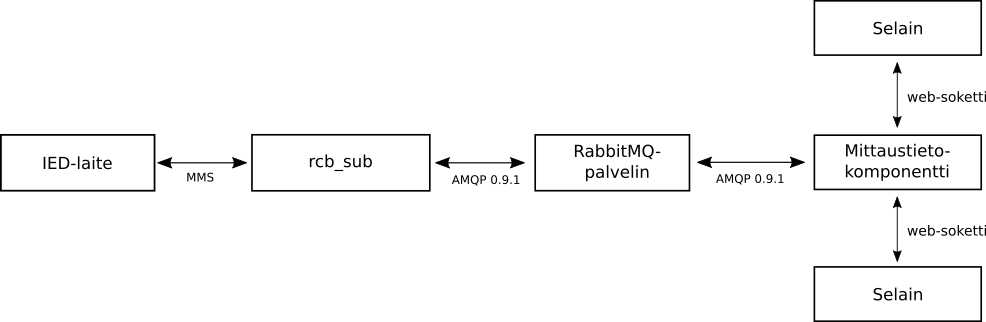
\includegraphics[width=1\textwidth]{pictures/example-use-case.png}
	\caption{Esimerkkikäyttötapaus, jossa mittaustietoa tilaava komponentti lähettää tietoa selaimen käyttöliittymään web-soketin avulla.}
	\label{fig:example-use-case}
\end{figure}


\section{Suorituskyky ja kielen valinta}
Ennen koko ohjelman uudelleenkirjoitusta, kokeiltiin demoa korjata vaihtamalla Ruby-tulkkia. Rubyn oletustulkki yritettiin vaihtaa \emph{JRuby}-tulkkiin \cite{jruby-homepage}. Tavoitteena vaihdossa oli saada Ruby-ohjelma toimimaan ilman globaalia tulkkilukitusta (GIL). JRuby on Ruby-tulkki, joka suorittaa Ruby-koodia \emph{Java-virtuaalikoneen} (engl. \emph{Java Virtual Machine}, lyhennetään \emph{JVM}) päällä. JRuby mahdollistaa säikeiden suorituksen rinnakkain JVM:n omilla säikeillä ja näin ollen suorituksen pitäisi olla nopeampaa \mbox{\cite{Youssef2013}}. Aidolla rinnakkaisuudella ohjelman suoritus ei olisi pysähtynyt viestin saapuessa takaisinkutsufunktion suorituksen ajaksi. Tämä ei vielä olisi kuitenkaan ratkaissut kaikkia ohjelmassa olevia ongelmia, kuten muistivuotoa ja hitaampaa suorituskykyä verrattuna käännettävään kieleen. Tämä toteutus ei kuitenkaan toiminut, ja yrityksen jälkeen päätettiin palata suunnitelmaan kirjoittaa koko ohjelma uudestaan. JRuby ei myöskään tukenut kaikkia projektin käyttämiä kirjastoja. Seurauksena olisi ollut saman projektin ylläpitäminen kahdelle eri tulkille tai asennettavien kirjastojen erottaminen. Kaikkiaan oli helpompaa kirjoittaa ohjelma alusta toisella tekniikalla.

Uuden toteutuksen kieleksi valittiin C-kieli. Isona syynä kielen valintaan oli tekijän iso mieltymys matalan tason ohjelmointiin ja C-kieleen. Lisäksi C-kieli käännetään alustalle suoraan konekäskyiksi, joiden suoritus on nopeampaa kuin tulkattavan kielen, kuten Ruby ja Python. Kielen valinnan yhteydessä varmistettiin kaikkien suunniteltujen liitosten mahdollisuus. C-kielelle löytyi kirjastoja RabbitMQ-välittäjäpalvelimen käyttämiseen ja lisäksi JSON-rakenteen muodostamiseen. Hyötynä vielä C-kielen valinnasta oli, että demossa käytettyä libIEC61850-kirjastoa pystyttiin käyttämään suoraan ilman erillistä liitosta, koska kirjasto oli myös tehty C-kielellä. Tarkemmin käytettyihin kirjastoihin mennään toteutuksessa.


\section{Prosessoidun viestin muoto ja rakenne}
% TODO: Kirjoita tästä eteenpäin oikein.
Saapuva viesti esitetään libIEC61850-kirjastossa \emph{ClientReport}-struk\-tuu\-rin instanssina. Se sisältää viestin datan ja sen voi lukea käyttämällä kirjaston tarjoamia funktioita \cite{libIEC61850-doc}. Saapunut viesti haluttiin jakaa välittäjäpalvelimen läpi muille osapuolille, joten viestin täytyi olla tekniikasta riippumattomassa muodossa. Hajautetuissa järjestelmissä viestin muoto muuttamalla tekniikasta riippumattomaksi saadaan aikaan joustavuutta osapuolten välille ja vähennetään osapuolten välistä riippuvuutta \cite[s.~838]{distributed-systems-concepts-and-design}. Viesti päädyttiin muuttamaan JSON-rakenteeksi. JSON-rakenteen voi helposti ihminen lukea ja se on nykypäivänä paljon käytetty tiedonsiirtomuoto erilaisissa web-palveluissa ja rajapinnoissa. Myöskin JSON-rakenteiden lukemiseen on monelle eri kielellä olemassa valmiita kirjastoja sen monikäyttöisyyden takia \mbox{\cite{Patrizio2016}}.

Liitteessä \ref{ch:report-json-format} on esitetty C-ohjelman viestistä muodostettu JSON-rakente. Saman JSON:in C-ohjelmaa julkaisi RabbitMQ-välittäjäpalvelimelle. Standardin määrittämää viestin rakennetta ja sisältöä käytiin läpi kappaleessa \ref{ch:viestin-rakenne}. JSON:in rakenne noudattaa pääosin standardin määrittämää viestin rakennetta. C-ohjelma lisäsi viestiin attribuuteihin sen viitteen, tyypin ja koon. Nämä tiedot eivät ole standardin määrittämässä viestissä ja ne todettiin tarpeelliseksi tiedoksi muille järjestelmän osille jotka viestejä lukevat. Tiedot luetaan ja selvitetään IED-laitteelta erillisillä palvelukutsuilla ennen tilauksen aloittamista. Nämä tiedot yhdistetään viestin saapuessa JSON-rakenteeseen. Tätä käsitellään tarkemmin kappaleessa \ref{ch:toteutus}.

Standardin viestin kenttien määrää pystyi säätämään RCB-instanssin \emph{OptFlds}-attribuutilla. JSON:iin kuitenkin haluttiin lisätä kaikki mahdolliset kentät selkeyden vuoksi. Jos kenttä puuttui viestistä, asetettiin sen arvoksi JSON:issa \emph{null}-arvo. Esimerkiksi liitteessä \ref{ch:report-json-format} kentän confRevision arvo on null. Tällöin RCB-instanssissa OptFlds-attribuutin \emph{conf-revision}-bitti on ollut epätosi. Sama toistettiin kaikille muillekin vaihtoehtoisille kentille. Tällä periaatteella viestin OptFlds-kenttä voitiin jättää pois JSON:ista. JSON:iin päädyttiin lisäämään FCD- ja FCDA-viitteisiin sisällytetyt oikeat attribuutien viitteet, tyyppit ja koot. Näin voidaan päätellä mitkä arvot oikeasti kuuluvat viestiin ja mitkä ovat niiden viitteet. Standardissa viesti sisälsi vain datajoukon FCD- tai FCDA-viitteen ja taulukon arvoja mihin attribuutteihin sen alla viitattiin. JSON:iin tämä taulukon arvot on avattu ja jokaiselle taulukon arvolle on lisätty sen viite, tyyppi ja koko. Liitteessä \ref{ch:report-json-format} oleva JSON-rakenne koostuu kahdesta sisäkkäisestä values-taulukosta (rivit 7 ja 13). Rivillä 7 oleva values-taulukko sisältää viestissä olevat datajoukon FCD- tai FCDA-viitteet ja niihin liittyvät kentät. Samalla periaatteella, kuin standardin määrittämässä viestin rakenteessa taulukon arvot 1--n:ään (kuva \ref{fig:iec61850-report-format}). Eli viestin \emph{Reason Code} on laitettu \emph{reasonForInclusion} attribuuttiin. Viestin \emph{DataRef}-kenttä on pilkottu kolmeen eri kenttään \emph{mmsReference}, \emph{reference} ja \emph{functionalConstraint}. Viestien viitteet tulevat MMS-protokollamäärityksen muodossa, eli pisteet (.) on korvattu dollari-merkillä (\$) ja viite sisältää funktionaalisen rajoitteen. Nyt mmsReference sisältää viestin alkuperäisen MMS-viitteen, reference sisältää standardin abstraktin viitteen ja functionalConstraint sisältää funktionaalisen rajoitteen. Nämä on erotettu selkeyden takia, koska mahdollisesti jotkin komponentit saattavat tarvita standardin käyttämää abstraktia viitettä ja näin välttää teksimuunnokset. JSON:in sisempi values-attribuutti (liitteessä \ref{ch:report-json-format} ensimmäinen rivillä 13) sisältää viestistä avatun arvo-taulukon. Jokaisen taulukon arvoon on lisätty sen koko viite, tyyppi ja koko. Poikkeuksena ovat \emph{boolean} ja \emph{utc-time} tyypit, joilla ei ole kokoa. Koko kertoo monellako bitillä kyseinen attribuutti esitetään, ja se voi vaihdella saman tyypin välillä, esimerkiksi \emph{bit-string}. Myöskin bit-string-tyypille päädyttiin lisäämään kaksi eri arvoa \emph{valueLittleEndian} ja \emph{valueBigEndian}. Attribuutista riippuen, sen tavujärjestys voi olla eri. Tämän takia päätettiin tarjota tilaajalle molemmat vaihtoehdot. Ajat päätettiin antaa suoraan samassa formaatissa kuin viestissä. Viestin päätason aikaleima on millisekunteja \emph{UNIX}-ajanlaskun alusta 1. tammikuuta 1970 klo 00:00:00 UTC tähän hetkeen. Attribuuteissa tyypiltään utc-time, luku on sekunteja samasta UNIX-ajanlaskusta tähän hetkeen \mbox{\cite[s.~26--27]{IEC61850-7-2}}.

Tutkimuskysymykseen jossa etsittiin vastausta kysymykseen mikä olisi sopiva tiedon jakamisen muoto hajautetussa järjestelmässä. Vastauksena kysymykseen tässä työssä valittiin JSON. JSON on nykypäivänä web-ohjelmoinnissa paljon käytetty tiedon jakamisen muoto rajapinnoissa. Toinen vaihtoehto olisi ollut XML-muoto, mutta se on raskaampi kuin JSON ja ei niin helposti ihmisen luettavissa \cite[s.~159]{distributed-systems-concepts-and-design}. JSON on ihmiselle helposti luettava ja ymmärrettävä muoto. JSON:in lukuun on olemassa monelle eri kielelle valmiita kirjastoja sen yleisyyden takia. JSON on myös kasvattanut suosiotaan ajan saatossa verrattuna XML:lään \cite{google-trends-xml-json}. JSON:in valinta todettiin hyväksi ja toimivaksi ratkaisuksi. \cite{the-rise-and-rise-of-json, why-json-is-better-than-xml}